\documentclass[border=2pt]{standalone}

\usepackage{pgf}
\usepackage{tikz}
\usepackage{notomath}
\usetikzlibrary{arrows,automata,positioning}
% \usepackage{geometry}

% \geometry{
%     letterpaper,
%     % total={170mm,257mm},
%     left=0.5in,
%     right=0.5in,
%     top=0.5in,
%     bottom=0.75in
% }


\begin{document}

\pagestyle{empty}

\centering

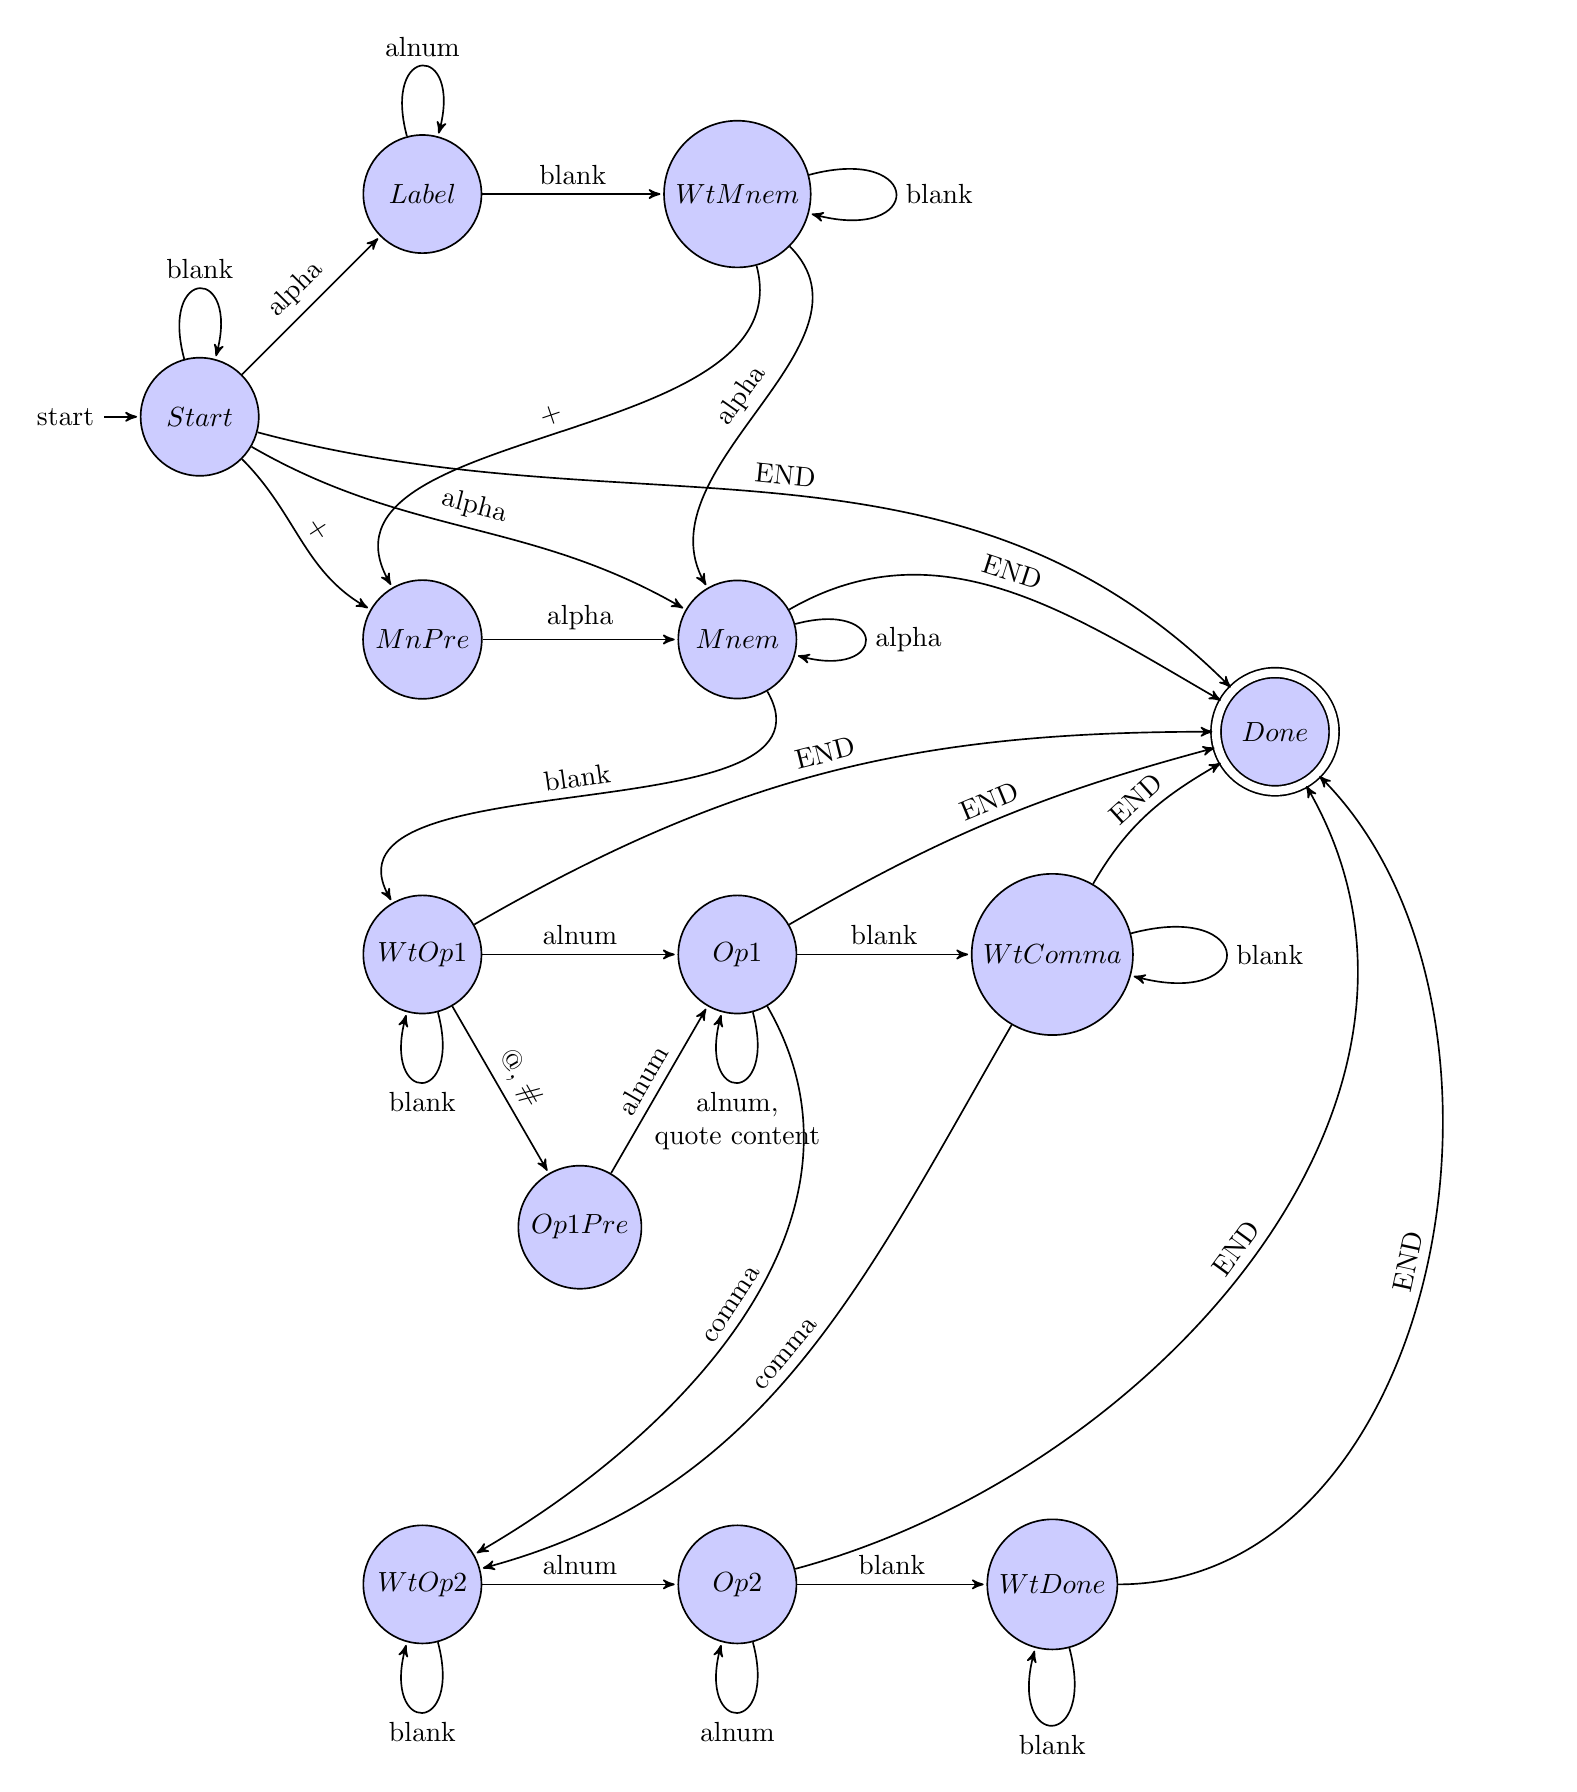
\begin{tikzpicture} [
        every state/.style={fill=blue!20, draw=black, minimum size=1.5cm},
        ->, >=stealth', shorten >=1pt, auto, node distance=4cm, semithick,
        accepting/.style={double, double distance=3pt},
        ->, >=stealth', auto, node distance=4cm, semithick
    ]
    % \tikzstyle{every state}=[fill=blue!20,draw=black,text=black]

    \node[initial,state]    (1)                         {$Start$};
    \node[state]            (2)  [above right of = 1]   {$Label$};
    \node[state]            (3)  [right of = 2]         {$WtMnem$};
    \node[state]            (4)  [below right of = 1]   {$MnPre$};
    \node[state]            (5)  [right of = 4]         {$Mnem$};

    \node[state]            (6)  [below of = 4]         {$WtOp1$};
    \node[state]            (7)  [right of = 6]         {$Op1$};
    \path (6) -- node[coordinate] (mid67) {} (7);
    \node[state]            (13) [below of=mid67, node distance=3.464cm]    {$Op1Pre$};
    \node[state]            (8)  [right of = 7]         {$WtComma$};

    \node[coordinate]       (14) [below of = 6]         {};
    \node[state]            (9)  [below of = 14]        {$WtOp2$};
    \node[state]            (10) [right of = 9]         {$Op2$};
    \node[state]            (12) [right of = 10]        {$WtDone$};

    \node[state, accepting] (11) [above right of = 8]   {$Done$};

    \path
    (1) % Start
    edge    [loop above]                                    node {blank}    (1)
    edge    [sloped, anchor=center, above]                  node {alpha}    (2)
    edge    [sloped, anchor=center, above, in=150, out=330] node {alpha}    (5)
    edge    [sloped, anchor=center, above, in=150, out=315] node {+}        (4)
    edge    [sloped, anchor=center, above, in=135, out=345] node {END}      (11)

    (2) % Label
    edge    [loop above]                                    node {alnum}    (2)
    edge    [sloped, anchor=center, above]                  node {blank}    (3)

    (3) % WtMnem
    edge    [loop right]                                    node {blank}    (3)
    edge    [sloped, anchor=center, above, in=120, out=285] node {+}        (4)
    edge    [sloped, anchor=center, above, in=120, out=315] node {alpha}    (5)

    (4) % MPre
    edge    [sloped, anchor=center, above]                  node {alpha}    (5)

    (5) % Mnem
    edge    [loop right]                                    node {alpha}    (5)
    edge    [sloped, anchor=center, above, in=120, out=300] node {blank}    (6)
    edge    [sloped, anchor=center, above, in=150, out=30]  node {END}      (11)

    (6) % WtOp1
    edge    [loop below]                                    node {blank}    (6)
    edge    [sloped, anchor=center, above]                  node {alnum}    (7)
    edge    [sloped, anchor=center, above, in=120, out=300] node {@, \#}    (13)
    edge    [sloped, anchor=center, above, in=180, out=30]  node {END}      (11)

    (13) % Op1Pre
    edge    [sloped, anchor=center, above, in=240, out=60]  node {alnum}    (7)

    (7) % Op1
    edge    [loop below, align=center]                      node {alnum,\\ quote content}    (7)
    edge    [sloped, anchor=center, above]                  node {blank}    (8)
    edge    [sloped, anchor=center, above, in=30, out=300]  node {comma}    (9)
    edge    [sloped, anchor=center, above, in=195, out=30]  node {END}      (11)

    (8) % WtComma
    edge    [loop right]                                    node {blank}    (8)
    edge    [sloped, anchor=center, above, in=15, out=240]  node {comma}    (9)
    edge    [sloped, anchor=center, above, in=210, out=60]  node {END}      (11)

    (9) % WtOp2
    edge    [loop below]                                    node {blank}    (9)
    edge    [sloped, anchor=center, above]                  node {alnum}    (10)

    (10) % Op2
    edge    [loop below]                                    node {alnum}    (10)
    edge    [sloped, anchor=center, above]                  node {blank}    (12)
    edge    [sloped, anchor=center, above, in=300, out=15]  node {END}   (11)

    (12) % WtDone
    edge    [loop below]                                    node {blank}    (12)
    edge    [sloped, anchor=center, above, in=315, out=0]   node {END}      (11);
\end{tikzpicture}


% \newpage


% \begin{tikzpicture} [state/.style=state with output, ->,>=stealth',shorten >=1pt,auto,node distance=5.0cm, semithick]

%     \tikzstyle{every state}=[fill=blue!20,draw=black,text=black]

%     \node[initial,state]	(1) 						{$1$ \nodepart{lower} $Retracting$};
%     \node[state]			(2) [above right of=1]		{$2$ \nodepart{lower} $Retracted$};
%     \node[state]			(3) [below right of=2]		{$3$ \nodepart{lower} $Extending$};
%     \node[state]			(4) [below left of=3]		{$4$ \nodepart{lower} $Extended$};
%     \node[state]			(5) [below of=4]			{$5$ \nodepart{lower} $Fault$};

%     \path	(1)	edge	[sloped, anchor=center, above]										node {xSenRet}				(2)
%     edge	[sloped, anchor=center, below, in=200, out=-20]						node {$xEN$}				(3)
%     edge	[sloped, anchor=center, below, bend right]							node {t $>$ timeMove}		(5)

%     (2) edge	[sloped, anchor=center, above]										node {xEn}					(3)
%     edge	[sloped, anchor=center, below, min distance=7cm, in=10, out=-10]	node {$\overline{xSenRet}$}	(5)

%     (3) edge	[sloped, anchor=center, above]										node {xSenExt}				(4)
%     edge	[sloped, anchor=center, above, in=20, out=160]						node {$\overline{xEN}$}		(1)
%     edge	[sloped, anchor=center, below, bend left]							node {t $>$ timeMove}		(5)

%     (4) edge	[sloped, anchor=center, above]										node {$\overline{xEN}$}		(1)
%     edge	[sloped, anchor=center, below]										node {$\overline{xSenExt}$}	(5)

%     (5) edge    [sloped, anchor=center, below, min distance=2.5cm, in=230, out=170]	node {xReset}				(1)

%     ; % Don't forget this semicolon

% \end{tikzpicture}


\end{document}